\section{Visualization}

\begin{figure}[t]
\begin{center}
\leavevmode
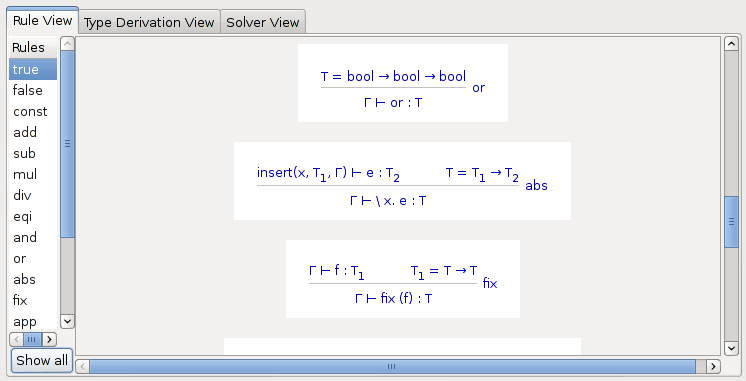
\includegraphics[width=\textwidth]{Figures/ruleview.png}
\end{center}
\caption{Rule View}
\label{fig:ruleview}
\end{figure}

To support the user of our library during the development of the type
checking phase, we implemented functionality to visualize the
constraint generation and the constraint solving process. Using this
visualization tool helps the developer to understand the derived type
checker in a more abstract way by allowing him to trace the type
derivation and the used solvers in a fine grained manner.

To implement such a tool a sufficient framework for graphical user
interfaces was needed. We wanted to implement this tool in
\textsc{Haskell}, so the library could be used directly without calls
from another language like \textsc{C}, thus a \textsc{Haskell} binding
for this toolkit was necessary. The second important criterion was
cross-platform support.

Since the number of well documented, stable bindings of gui frameworks
for \textsc{Haskell} that work cross-platform is rather limited, the
choice came down to \textit{wxHaskell~(wxWidgets)}~\cite{wxWidgets}
and \textit{Gtk2Hs~(Gtk)}~\cite{gtk}. Both frameworks are mature and
widely used. \textit{Gtk} provides the gui interface builder
\textit{Glade}, which tipped the favor towards \textit{Gtk2Hs} to
implement the graphical user interface of the tool.

As part of the tool design we identified three main work flows which
should be supported accordingly. At first, the user should be able to
get a concise overview of the typing rules he implemented using the
library's EDSL, thus the tool must provide a sufficient rendering of
the defined deduction rules. Secondly, the tool should allow the user
to trace the library's constraint generation algorithm by rendering
the derivation tree for a given expression and thus giving the user
the opportunity to understand which rules have been instantiated and
which constraints have been collected. Last but not least the tool
should allow the user to trace the constraint solving process step by
step.

To capture these requirements we designed three main views within the
tool: the \textit{Rule View}, the \textit{Type Derivation View}, and
the \textit{Solver View}. The \textit{Rule View} provides a ``pretty''
rendering of the user's type system, the \textit{Type Derivation View}
renders the type derivation tree of a given expression, and the
\textit{Solver View} is basically a step-by-step trace of the used
solvers.

The graphical user interface of the tool was developed with the help
of \textit{Gtk}'s gui designer \textit{Glade}. To gather all
information needed for the visualization of the different phases, the
constraint generation and the constraint solving algorithms had to be
adapted slightly. The core algorithms are still the same but the
generation and solving process is documented with additional
informations in separate data structures for the visualization
purpose. The constraint generation algorithm returns a plain list of
constraints, neglecting the tree structure which reflects the
dependencies and order of the generation process. But since that is
exactly what we want to show in the \textit{Type Derivation View} the
implementation now returns the normal list but also a tree in which
all these informations are stored.

In the implementation of the constraint solving algorithm we
introduced a data structure which stores in each solving step the
current constraint, the solution of that constraint, the accumulated
result substitution, and the constraints jet to be solved:

\begin{lstlisting}
data IntermediateResult =
    IRes { con   :: Judgement    -- current constraint
         , res   :: Result       -- solution of constraint
         , subs  :: Substitution -- acc. result substitution
         , unsolv:: [Judgement]  -- remaining constraints
         }
\end{lstlisting}

A list of these intermediate results is than returned along the proper
result allowing to trace step-by-step through the constraint solving
process.

With these modifications we are able to visualize the inner machinery
of our framework. To get a better feeling, what such a derived tool
could look like, let us take a closer look on the gui-based inspector
tool derived for our \textsc{MiniML} example.

The \textit{Rule View} (Fig.~\ref{fig:ruleview}) displays the
constraint-based deduction rules defined as part of \textsc{MiniML}'s
inference system in a more readable manner. The left side of the view
is a list, where a rule can be selected to be displayed on the
right. Under that list is a button to display all rules, one below the
other, on the right side.

\begin{figure}[t]
\begin{center}
\leavevmode
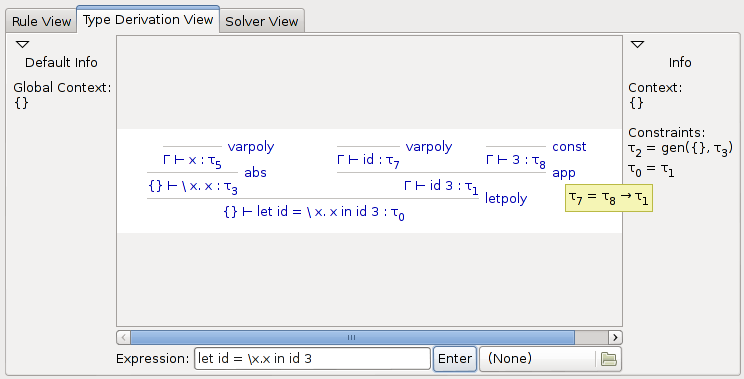
\includegraphics[width=\textwidth]{Figures/typeview.png}
\end{center}
\caption{Type Derivation View}
\label{fig:typeview}
\end{figure}

The \textit{Type Derivation View} generates the internal derivation
tree for an expression entered at the bottom text field. Let us
consider for example the expression ``\texttt{let id = \textbackslash
  x.x in id 3}'', whose derivation tree is shown in
Fig.~\ref{fig:typeview}.

The derivation tree of our example expression is displayed right above
the text field. On the left of the tree the global information for the
type checking process are displayed, at the moment this is only the
global context which is passed on to the constraint solvers. The
derivation tree contains only judgements, no constraints. To view the
constraints the user can hover with the mouse over the rule name, to
get a tooltip with the constraints or he can click on the rule
name. Clicking on the rule name will fill the right side with
information about that rule instance, namely the local context and the
constraints arising from this rule.

\begin{figure}[t]
\begin{center}
\leavevmode
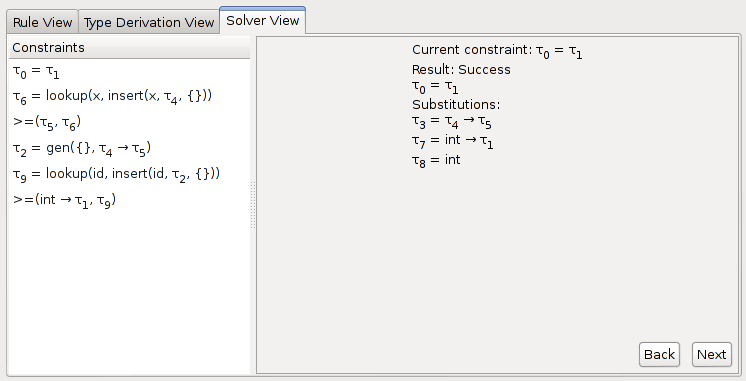
\includegraphics[width=\textwidth]{Figures/solverview.png}
\end{center}
\caption{Solver View}
\label{fig:solverview}
\end{figure}

The last view is the \textit{Solver View}. In this view the user can
step through the constraint solving process.  The left side lists the
constraints yet to be solved. The right side displays the current
constraint considered by the solver, the solution of that constraint
and the accumulated result substitution. At the bottom right side are
the two buttons to step through the solving process.

\bigskip

To run this gui tool, the user needs to provide three things: a list
of named inference rules, an initial global context and a function to
parse expressions. For our \textsc{MiniML} example the tool could be
run as following:

\begin{lstlisting}
main = runGui GuiConfig { namedRules    = rules
                        , globalContext = empty
                        , parseString   = parse
                        }

rules :: [(String,Rule)]
rules = [ ("true", true)
        , ("false", false)
        , ("letrec", letrec)
        , ("varpoly", varpoly)
        , (...) ]
\end{lstlisting}
